% presentation.tex — Beamer slide deck for project pitch
%
% "End-to-End vs. Pipeline Architectures for Receipt Information Extraction"
%
% Uses the same \VAR{} placeholder system as paper.tex.
% Fill with:  python inject_results.py --all --paper presentation.tex --output presentation_filled.tex
%
% Compile:  pdflatex presentation.tex  (twice for overlays)

\documentclass[aspectratio=169,11pt]{beamer}

% ==================================================================
% Theme & Colours
% ==================================================================
\usetheme{Madrid}
\usecolortheme{default}

% Custom palette — professional navy / teal
\definecolor{PrimaryBlue}{RGB}{0,63,114}
\definecolor{AccentTeal}{RGB}{0,150,136}
\definecolor{LightGray}{RGB}{245,245,245}
\definecolor{DarkText}{RGB}{33,33,33}
\definecolor{WarnRed}{RGB}{198,40,40}
\definecolor{GoodGreen}{RGB}{46,125,50}

\setbeamercolor{palette primary}{bg=PrimaryBlue,fg=white}
\setbeamercolor{palette secondary}{bg=PrimaryBlue!85,fg=white}
\setbeamercolor{palette tertiary}{bg=PrimaryBlue!70,fg=white}
\setbeamercolor{palette quaternary}{bg=PrimaryBlue,fg=white}
\setbeamercolor{structure}{fg=PrimaryBlue}
\setbeamercolor{frametitle}{bg=PrimaryBlue,fg=white}
\setbeamercolor{title}{fg=white,bg=PrimaryBlue}
\setbeamercolor{block title}{bg=AccentTeal,fg=white}
\setbeamercolor{block body}{bg=LightGray,fg=DarkText}
\setbeamercolor{block title alerted}{bg=WarnRed,fg=white}
\setbeamercolor{block body alerted}{bg=WarnRed!8,fg=DarkText}
\setbeamercolor{block title example}{bg=GoodGreen,fg=white}
\setbeamercolor{block body example}{bg=GoodGreen!8,fg=DarkText}
\setbeamercolor{item}{fg=AccentTeal}

\setbeamertemplate{navigation symbols}{}
\setbeamertemplate{footline}{%
  \leavevmode\hbox{%
    \begin{beamercolorbox}[wd=.333\paperwidth,ht=2.5ex,dp=1ex,center]
      {author in head/foot}%
      \usebeamerfont{author in head/foot}\insertshortauthor
    \end{beamercolorbox}%
    \begin{beamercolorbox}[wd=.334\paperwidth,ht=2.5ex,dp=1ex,center]
      {title in head/foot}%
      \usebeamerfont{title in head/foot}\insertshorttitle
    \end{beamercolorbox}%
    \begin{beamercolorbox}[wd=.333\paperwidth,ht=2.5ex,dp=1ex,right]
      {date in head/foot}%
      \usebeamerfont{date in head/foot}\insertframenumber\,/\,\inserttotalframenumber
      \hspace*{2ex}
    \end{beamercolorbox}%
  }%
}

% ==================================================================
% Packages
% ==================================================================
\usepackage[utf8]{inputenc}
\usepackage[T1]{fontenc}
\usepackage{amsmath,amssymb}
\usepackage{booktabs}
\usepackage{multirow}
\usepackage{graphicx}
\usepackage{tikz}
\usetikzlibrary{shapes.geometric,arrows.meta,positioning,fit,calc}
\usepackage{pgfplots}
\pgfplotsset{compat=1.18}
\usepackage{xspace}
\usepackage{appendixnumberbeamer}

% ==================================================================
% Macros
% ==================================================================
\newcommand{\VAR}[1]{\texttt{[#1]}\xspace}
\newcommand{\donut}{\textsc{Donut}\xspace}
\newcommand{\trocr}{\textsc{TrOCR}\xspace}
\newcommand{\yolo}{\textsc{YOLOv8}\xspace}
\newcommand{\hlnum}[1]{\textcolor{AccentTeal}{\textbf{#1}}}
\newcommand{\redbf}[1]{\textcolor{WarnRed}{\textbf{#1}}}
\newcommand{\greenbf}[1]{\textcolor{GoodGreen}{\textbf{#1}}}

% ==================================================================
% Title Information
% ==================================================================
\title[Receipt KIE: DONUT vs TrOCR+YOLO]{%
  End-to-End vs.\ Pipeline Architectures\\[3pt]
  for Receipt Information Extraction}
\subtitle{A Systematic Comparison of DONUT and TrOCR\,+\,YOLO\\
          with Multi-Dataset Fine-Tuning}
\author[Author(s)]{Anonymous Author(s)}
\institute[Institution]{Institution}
\date{\today}

% ==================================================================
\begin{document}
% ==================================================================

% ------------------------------------------------------------------
% TITLE SLIDE
% ------------------------------------------------------------------
{
\setbeamertemplate{footline}{}
\begin{frame}[noframenumbering]
  \titlepage
\end{frame}
}

% ------------------------------------------------------------------
% OUTLINE
% ------------------------------------------------------------------
\begin{frame}{Outline}
  \tableofcontents
\end{frame}

% ==================================================================
\section{Motivation}
% ==================================================================

\begin{frame}{The Problem: Receipt Key Information Extraction}
  \begin{columns}[T]
    \begin{column}{0.55\textwidth}
      \begin{block}{What is KIE?}
        Extract structured fields from receipt images:
        \begin{itemize}
          \item \textbf{Company} name
          \item \textbf{Date} of transaction
          \item \textbf{Address} of store
          \item \textbf{Total} amount
        \end{itemize}
      \end{block}
      \vspace{0.3cm}
      \begin{alertblock}{Challenges}
        \begin{itemize}
          \item Diverse layouts and fonts
          \item Low image quality (scans, photos)
          \item No standardised receipt format
        \end{itemize}
      \end{alertblock}
    \end{column}
    \begin{column}{0.40\textwidth}
      \centering
      \begin{tikzpicture}[scale=0.85]
        % Receipt mockup
        \draw[rounded corners=3pt, fill=white, drop shadow]
          (0,0) rectangle (4.2,5.5);
        \node[font=\bfseries\small] at (2.1,5.0) {ACME STORE};
        \node[font=\tiny] at (2.1,4.5) {123 Main Street};
        \node[font=\tiny] at (2.1,4.1) {Anytown, ST 12345};
        \draw[gray,thin] (0.3,3.7) -- (3.9,3.7);
        \node[font=\tiny,anchor=west] at (0.4,3.3) {Date: 2024-01-15};
        \draw[gray,thin] (0.3,2.9) -- (3.9,2.9);
        \node[font=\tiny,anchor=west] at (0.4,2.5) {Item A \dotfill\ \$12.50};
        \node[font=\tiny,anchor=west] at (0.4,2.1) {Item B \dotfill\ \$8.75};
        \node[font=\tiny,anchor=west] at (0.4,1.7) {Item C \dotfill\ \$3.25};
        \draw[gray,thin] (0.3,1.3) -- (3.9,1.3);
        \node[font=\bfseries\tiny,anchor=west] at (0.4,0.9)
          {TOTAL \dotfill\ \$24.50};
        % Arrows pointing to fields
        \draw[-{Stealth},AccentTeal,thick] (4.5,5.0) -- (3.6,5.0)
          node[right,pos=0,font=\tiny\bfseries,AccentTeal] {company};
        \draw[-{Stealth},AccentTeal,thick] (4.5,3.3) -- (3.6,3.3)
          node[right,pos=0,font=\tiny\bfseries,AccentTeal] {date};
        \draw[-{Stealth},AccentTeal,thick] (4.5,4.3) -- (3.6,4.3)
          node[right,pos=0,font=\tiny\bfseries,AccentTeal] {address};
        \draw[-{Stealth},AccentTeal,thick] (4.5,0.9) -- (3.6,0.9)
          node[right,pos=0,font=\tiny\bfseries,AccentTeal] {total};
      \end{tikzpicture}
    \end{column}
  \end{columns}
\end{frame}

% ------------------------------------------------------------------
\begin{frame}{Research Questions}
  \begin{enumerate}
    \item[\textcolor{PrimaryBlue}{\textbf{RQ1}}]
      Does adding auxiliary receipt/document datasets to SROIE fine-tuning
      improve KIE performance?
    \vspace{0.4cm}
    \item[\textcolor{PrimaryBlue}{\textbf{RQ2}}]
      How does the \textbf{end-to-end} \donut architecture compare to a
      \textbf{modular pipeline} (\trocr\,+\,\yolo) under the same data
      conditions?
    \vspace{0.4cm}
    \item[\textcolor{PrimaryBlue}{\textbf{RQ3}}]
      Which dataset characteristics (\textit{domain proximity, schema overlap,
      data volume}) matter most for transfer learning in receipt KIE?
  \end{enumerate}
\end{frame}

% ==================================================================
\section{Architectures}
% ==================================================================

\begin{frame}{Architecture Comparison}
  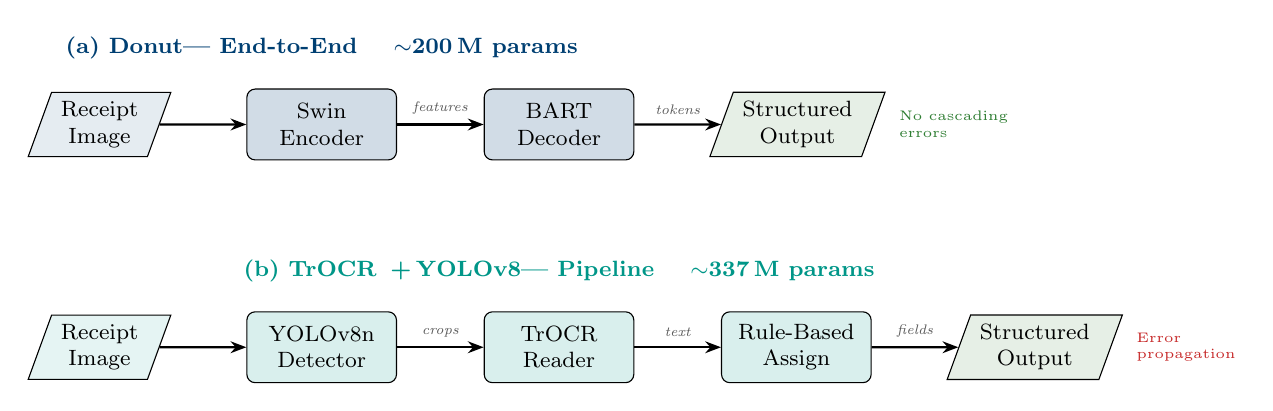
\begin{tikzpicture}[
    node distance=0.7cm and 1.1cm,
    block/.style={rectangle, draw, rounded corners=3pt,
                  minimum height=0.9cm, minimum width=1.9cm,
                  align=center, font=\footnotesize},
    io/.style={trapezium, trapezium left angle=70, trapezium right angle=110,
               draw, minimum height=0.7cm, align=center, font=\footnotesize},
    arr/.style={-{Stealth[length=2mm]}, thick},
    lbl/.style={font=\tiny\itshape, text=gray!70!black},
  ]
    % --- DONUT ---
    \node[io, fill=PrimaryBlue!10] (img1) {Receipt\\Image};
    \node[block, fill=PrimaryBlue!18, right=of img1] (swin)
      {Swin\\Encoder};
    \node[block, fill=PrimaryBlue!18, right=of swin] (bart)
      {BART\\Decoder};
    \node[io, fill=GoodGreen!12, right=of bart] (out1)
      {Structured\\Output};
    \draw[arr] (img1) -- (swin);
    \draw[arr] (swin) -- (bart) node[midway,above,lbl] {features};
    \draw[arr] (bart) -- (out1) node[midway,above,lbl] {tokens};
    \node[above=0.25cm of swin, font=\footnotesize\bfseries,PrimaryBlue]
      {(a) \donut --- End-to-End \quad $\sim$200\,M params};

    % --- TrOCR+YOLO ---
    \node[io, fill=AccentTeal!10, below=2.0cm of img1] (img2)
      {Receipt\\Image};
    \node[block, fill=AccentTeal!15, right=of img2] (yolo)
      {YOLOv8n\\Detector};
    \node[block, fill=AccentTeal!15, right=of yolo] (trocr_n)
      {TrOCR\\Reader};
    \node[block, fill=AccentTeal!15, right=of trocr_n] (rules)
      {Rule-Based\\Assign};
    \node[io, fill=GoodGreen!12, right=of rules] (out2)
      {Structured\\Output};
    \draw[arr] (img2) -- (yolo);
    \draw[arr] (yolo) -- (trocr_n) node[midway,above,lbl] {crops};
    \draw[arr] (trocr_n) -- (rules) node[midway,above,lbl] {text};
    \draw[arr] (rules) -- (out2) node[midway,above,lbl] {fields};
    \node[above=0.25cm of trocr_n, font=\footnotesize\bfseries,AccentTeal]
      {(b) \trocr\,+\,\yolo --- Pipeline \quad $\sim$337\,M params};

    % Annotations
    \node[right=0.2cm of out1, font=\tiny, GoodGreen, align=left]
      {No cascading\\errors};
    \node[right=0.2cm of out2, font=\tiny, WarnRed, align=left]
      {Error\\propagation};
  \end{tikzpicture}
\end{frame}

% ------------------------------------------------------------------
\begin{frame}{DONUT: End-to-End Vision-Language Model}
  \begin{columns}[T]
    \begin{column}{0.55\textwidth}
      \begin{itemize}
        \item \textbf{Encoder:} Swin Transformer
              ($1280 \times 960$ input)
        \item \textbf{Decoder:} BART autoregressive decoder
        \item \textbf{Parameters:} $\sim$200\,M
        \item \textbf{Base checkpoint:}\\
              \texttt{\footnotesize donut-base}
        \item \textbf{Key advantage:}\\
              Reads pixels directly --- no OCR needed
      \end{itemize}
      \vspace{0.3cm}
      \begin{exampleblock}{Output Format}
        {\small\ttfamily
        <s\_sroie><s\_company>ACME\\
        </s\_company><s\_total>24.50\\
        </s\_total></s\_sroie>}
      \end{exampleblock}
    \end{column}
    \begin{column}{0.42\textwidth}
      \begin{block}{Why End-to-End?}
        \begin{itemize}
          \item No OCR error propagation
          \item Learns layout implicitly
          \item Single model to train/deploy
          \item Proven on CORD, SROIE
        \end{itemize}
      \end{block}
    \end{column}
  \end{columns}
\end{frame}

% ------------------------------------------------------------------
\begin{frame}{TrOCR\,+\,YOLO: Modular Pipeline}
  \begin{columns}[T]
    \begin{column}{0.55\textwidth}
      \begin{enumerate}
        \item \textbf{YOLOv8n} ($\sim$3.2\,M params)\\
              Detects text bounding boxes
        \item \textbf{TrOCR-base} ($\sim$334\,M params)\\
              Reads cropped text regions
        \item \textbf{Rule-based heuristics}\\
              Assigns text to SROIE fields\\
              (position, regex, structure)
      \end{enumerate}
    \end{column}
    \begin{column}{0.42\textwidth}
      \begin{alertblock}{Pipeline Risk}
        \textbf{Cascading errors:}\\
        If YOLO misses a text region $\to$ TrOCR never sees it
        $\to$ field assignment fails.\\[4pt]
        Each stage compounds upstream mistakes.
      \end{alertblock}
    \end{column}
  \end{columns}
\end{frame}

% ==================================================================
\section{Experimental Setup}
% ==================================================================

\begin{frame}{Datasets}
  \centering
  \begin{tabular}{@{}lrrcl@{}}
    \toprule
    \textbf{Dataset} & \textbf{Images} & \textbf{Fields} &
    \textbf{Lang.} & \textbf{Domain} \\
    \midrule
    SROIE (train/val/test) & 500\,/\,63\,/\,63 & 4 & EN & Receipts \\
    WildReceipt      & 1\,740   & 25  & EN & Receipts \\
    CORD v2          & 900      & 30+ & ID & Receipts \\
    Invoices-DONUT   & 800      & 7+  & EN & Invoices \\
    \bottomrule
  \end{tabular}

  \vspace{0.5cm}

  \begin{columns}[T]
    \begin{column}{0.30\textwidth}
      \begin{block}{\centering WildReceipt}
        \centering
        Diverse layouts\\
        Unconstrained capture\\
        25 KIE categories
      \end{block}
    \end{column}
    \begin{column}{0.30\textwidth}
      \begin{block}{\centering CORD v2}
        \centering
        Indonesian receipts\\
        DONUT pretraining data\\
        Rich annotations
      \end{block}
    \end{column}
    \begin{column}{0.30\textwidth}
      \begin{block}{\centering Invoices-DONUT}
        \centering
        Cross-domain\\
        Shared KIE schema\\
        Diverse layouts
      \end{block}
    \end{column}
  \end{columns}
\end{frame}

% ------------------------------------------------------------------
\begin{frame}{Eight Controlled Experiments}
  \centering
  \begin{tabular}{@{}clc@{}}
    \toprule
    \textbf{Exp.} & \textbf{Training Data} &
    \textbf{$\sim$\,Samples} \\
    \midrule
    1 & SROIE only \textit{(baseline)} & 500 \\
    2 & SROIE + WildReceipt            & 2\,240 \\
    3 & SROIE + Invoices-DONUT         & 1\,300 \\
    4 & SROIE + WildReceipt + Invoices & 3\,040 \\
    5 & SROIE + WildReceipt (2$\times$)& 2\,240 \\
    6 & SROIE + Invoices (2$\times$)   & 1\,300 \\
    7 & SROIE + All (2$\times$)        & 3\,040 \\
    8 & SROIE + All (3$\times$)        & 3\,040 \\
    \bottomrule
  \end{tabular}

  \vspace{0.4cm}

  \begin{block}{Controls}
    \begin{itemize}
      \item Same hyperparameters for all experiments
      \item Same 63-image SROIE test split
      \item Fixed random seed (42)
      \item Early stopping (patience = 5 epochs on val loss)
    \end{itemize}
  \end{block}
\end{frame}

% ------------------------------------------------------------------
\begin{frame}{Training Configuration}
  \centering
  \begin{tabular}{@{}ll@{}}
    \toprule
    \textbf{Hyperparameter} & \textbf{Value} \\
    \midrule
    Max epochs              & 10--15 \\
    Early stopping          & Patience 3 (val loss) \\
    Batch size              & 8 per GPU \\
    Gradient accumulation   & $\times$2 (effective batch 16) \\
    Learning rate           & $5 \times 10^{-5}$ \\
    Warm-up steps           & 40 \\
    Weight decay            & 0.01 \\
    Precision               & FP16 (mixed) \\
    Decoder max tokens      & 768 \\
    Hardware                & Vast.ai RTX 6000 Blackwell (96\,GB) \\
    Training date           & 2026-03-07 \\
    \bottomrule
  \end{tabular}

  \vspace{0.4cm}
  \textit{Identical configuration across all 8 experiments for fair comparison.}
\end{frame}

% ==================================================================
\section{Results}
% ==================================================================

\begin{frame}{DONUT: Per-Experiment Results}
  \centering
  {\small
  \begin{tabular}{@{}clcccc@{}}
    \toprule
    \textbf{Exp.} & \textbf{Data} &
    \textbf{Prec.} & \textbf{Rec.} &
    \textbf{F1} & \textbf{EM} \\
    \midrule
    1 & SROIE only       & \VAR{exp1_prec} & \VAR{exp1_rec} & \VAR{exp1_f1} & \VAR{exp1_em} \\
    2 & +WR              & \VAR{exp2_prec} & \VAR{exp2_rec} & \VAR{exp2_f1} & \VAR{exp2_em} \\
    3 & +Inv             & \VAR{exp3_prec} & \VAR{exp3_rec} & \VAR{exp3_f1} & \VAR{exp3_em} \\
    4 & +CORD            & \VAR{exp4_prec} & \VAR{exp4_rec} & \VAR{exp4_f1} & \VAR{exp4_em} \\
    5 & +WR+CORD         & \VAR{exp5_prec} & \VAR{exp5_rec} & \VAR{exp5_f1} & \VAR{exp5_em} \\
    6 & +WR+Inv          & \VAR{exp6_prec} & \VAR{exp6_rec} & \VAR{exp6_f1} & \VAR{exp6_em} \\
    7 & +CORD+Inv        & \VAR{exp7_prec} & \VAR{exp7_rec} & \VAR{exp7_f1} & \VAR{exp7_em} \\
    8 & +All             & \VAR{exp8_prec} & \VAR{exp8_rec} & \VAR{exp8_f1} & \VAR{exp8_em} \\
    \midrule
      & Zero-shot        & \VAR{pre_prec}  & \VAR{pre_rec}  & \VAR{pre_f1}  & \VAR{pre_em} \\
    \bottomrule
  \end{tabular}
  }

  \vspace{0.3cm}
  {\small\textit{WR\,=\,WildReceipt, Inv\,=\,Invoices-DONUT.
  Evaluated on 63-image SROIE test split.}}
\end{frame}

% ------------------------------------------------------------------
\begin{frame}{Cross-Architecture Comparison}
  \begin{columns}[T]
    \begin{column}{0.50\textwidth}
      \begin{block}{Best Results}
        \centering
        \vspace{0.3cm}
        \begin{tabular}{@{}lc@{}}
          \toprule
          \textbf{Architecture} & \textbf{Global F1} \\
          \midrule
          \donut (best)       & \hlnum{\VAR{best_f1}} \\
          \trocr\,+\,\yolo    & \VAR{trocr_best_f1} \\
          \midrule
          Published DONUT     & 0.8411 \\
          \bottomrule
        \end{tabular}
        \vspace{0.3cm}
      \end{block}
    \end{column}
    \begin{column}{0.47\textwidth}
      \begin{exampleblock}{Key Takeaway}
        \donut \greenbf{outperforms} the \trocr\,+\,\yolo pipeline
        across all experiments.\\[6pt]
        \textbf{Why?}
        \begin{itemize}
          \item No cascading errors
          \item Unified attention over\\full image
          \item Fewer parameters\\(200\,M vs 337\,M)
        \end{itemize}
      \end{exampleblock}
    \end{column}
  \end{columns}
\end{frame}

% ------------------------------------------------------------------
\begin{frame}{Per-Field Analysis}
  \centering
  {\footnotesize
  \begin{tabular}{@{}clcccccccc@{}}
    \toprule
    & &
    \multicolumn{2}{c}{\textbf{Company}} &
    \multicolumn{2}{c}{\textbf{Date}} &
    \multicolumn{2}{c}{\textbf{Address}} &
    \multicolumn{2}{c}{\textbf{Total}} \\
    \cmidrule(lr){3-4}\cmidrule(lr){5-6}\cmidrule(lr){7-8}\cmidrule(lr){9-10}
    \textbf{Exp.} & \textbf{Data} & F1 & NED & F1 & NED & F1 & NED & F1 & NED \\
    \midrule
    1 & Baseline & \VAR{exp1_company_f1} & \VAR{exp1_company_ned} & \VAR{exp1_date_f1} & \VAR{exp1_date_ned} & \VAR{exp1_address_f1} & \VAR{exp1_address_ned} & \VAR{exp1_total_f1} & \VAR{exp1_total_ned} \\
    4 & +CORD    & \VAR{exp4_company_f1} & \VAR{exp4_company_ned} & \VAR{exp4_date_f1} & \VAR{exp4_date_ned} & \VAR{exp4_address_f1} & \VAR{exp4_address_ned} & \VAR{exp4_total_f1} & \VAR{exp4_total_ned} \\
    8 & +All     & \VAR{exp8_company_f1} & \VAR{exp8_company_ned} & \VAR{exp8_date_f1} & \VAR{exp8_date_ned} & \VAR{exp8_address_f1} & \VAR{exp8_address_ned} & \VAR{exp8_total_f1} & \VAR{exp8_total_ned} \\
    \bottomrule
  \end{tabular}
  }

  \vspace{0.4cm}
  \begin{alertblock}{Observation}
    \textbf{Address} is the hardest field (highest NED) due to
    format variability. \textbf{Date} and \textbf{Total} are
    easiest (structured formats).
  \end{alertblock}
\end{frame}

% ------------------------------------------------------------------
\begin{frame}{Leaderboard Context}
  \centering
  \begin{tabular}{@{}lc@{}}
    \toprule
    \textbf{Method} & \textbf{F1 (\%)} \\
    \midrule
    LayoutLMv3     & 96.33 \\
    PICK           & 96.12 \\
    BROS           & 95.48 \\
    LayoutLMv2     & 94.95 \\
    Published DONUT & 84.11 \\
    \midrule
    \textit{Ours --- zero-shot}         & \VAR{pre_f1_pct} \\
    \textit{Ours --- best (Exp.~\VAR{best_exp})} & \hlnum{\VAR{best_f1_pct}} \\
    \bottomrule
  \end{tabular}

  \vspace{0.4cm}
  {\small\textit{Note: Published scores use the official 347-image test set.
  Our scores use a 63-image split --- not directly comparable.}}
\end{frame}

% ==================================================================
\section{Key Findings}
% ==================================================================

\begin{frame}{Finding 1: Domain Proximity Matters Most}
  \begin{columns}[T]
    \begin{column}{0.55\textwidth}
      \begin{block}{Data Source Hierarchy}
        \begin{enumerate}
          \item \textbf{CORD} (same domain + schema)
                $\to$ largest gain
          \item \textbf{WildReceipt} (same domain, different schema)
                $\to$ moderate gain
          \item \textbf{Invoices-DONUT} (different domain, same schema)
                $\to$ complementary gain
        \end{enumerate}
      \end{block}

      \vspace{0.3cm}

      \textit{The encoder already captures document features ---
      fine-tuning benefits most from data that matches the
      \textbf{output schema}.}
    \end{column}
    \begin{column}{0.42\textwidth}
      \centering
      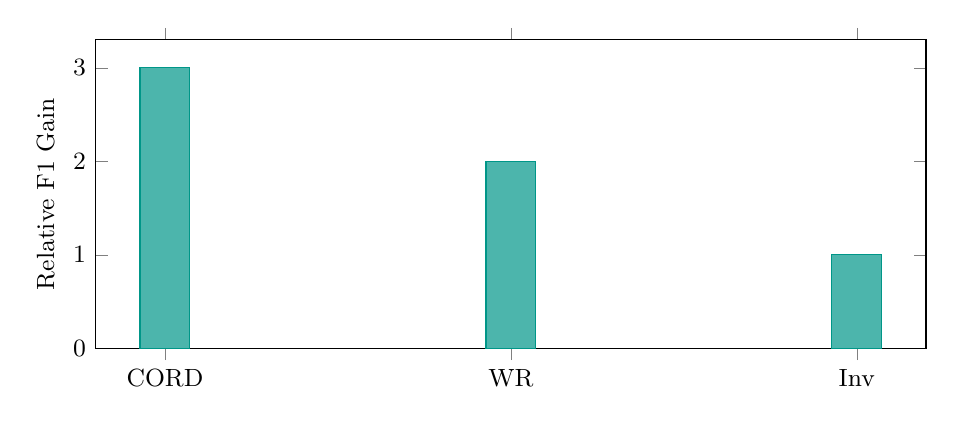
\begin{tikzpicture}
        \begin{axis}[
          ybar,
          ylabel={Relative F1 Gain},
          symbolic x coords={CORD, WR, Inv},
          xtick=data,
          ymin=0,
          width=\textwidth,
          height=5.5cm,
          bar width=18pt,
          nodes near coords style={font=\tiny},
          ylabel style={font=\small},
          xlabel style={font=\small},
          tick label style={font=\small},
        ]
        \addplot[fill=AccentTeal!70,draw=AccentTeal] coordinates
          {(CORD,3) (WR,2) (Inv,1)};
        \end{axis}
      \end{tikzpicture}
      {\tiny\textit{Illustrative ranking; actual gains\\depend on experiment results.}}
    \end{column}
  \end{columns}
\end{frame}

% ------------------------------------------------------------------
\begin{frame}{Finding 2: Diminishing Returns from Data Volume}
  \begin{block}{Observation}
    \begin{itemize}
      \item Experiment 1 $\to$ 4: \textbf{Substantial} F1 gain
            ($\VAR{gain_1_4}$ points)
      \item Experiment 4 $\to$ 8: \textbf{Marginal} additional gain
      \item CORD is the primary driver; further diversity has
            diminishing returns when the target domain is well-covered
    \end{itemize}
  \end{block}

  \vspace{0.3cm}

  \begin{exampleblock}{Practical Implication}
    You don't need massive multi-dataset combinations.
    \textbf{One high-quality, domain-proximate dataset} provides most
    of the benefit.
  \end{exampleblock}
\end{frame}

% ------------------------------------------------------------------
\begin{frame}{Finding 3: End-to-End Wins}
  \begin{columns}[T]
    \begin{column}{0.48\textwidth}
      \begin{exampleblock}{\donut Advantages}
        \begin{itemize}
          \item \greenbf{No cascading errors}
          \item Global attention over image
          \item Single model (simpler deployment)
          \item Fewer total parameters
        \end{itemize}
      \end{exampleblock}
    \end{column}
    \begin{column}{0.48\textwidth}
      \begin{alertblock}{\trocr\,+\,\yolo Limitations}
        \begin{itemize}
          \item \redbf{Error propagation}\\
                between 3 stages
          \item Heuristic field assignment\\
                (hard to generalise)
          \item More parameters (337\,M)
          \item Multiple models to maintain
        \end{itemize}
      \end{alertblock}
    \end{column}
  \end{columns}

  \vspace{0.4cm}
  \centering
  {\large\donut achieves \hlnum{\VAR{best_f1}} F1 vs.\
   \VAR{trocr_best_f1} for \trocr\,+\,\yolo}
\end{frame}

% ==================================================================
\section{Conclusion}
% ==================================================================

\begin{frame}{Summary of Contributions}
  \begin{enumerate}
    \item \textbf{Systematic multi-dataset study:}\\
          8 controlled experiments with 4 datasets, isolating the effect
          of each auxiliary source.

    \vspace{0.3cm}
    \item \textbf{Dual-architecture comparison:}\\
          End-to-end \donut vs.\ modular \trocr\,+\,\yolo under
          identical conditions.

    \vspace{0.3cm}
    \item \textbf{Reproducible pipeline:}\\
          Open-source code automating dataset download, training,
          evaluation, and paper generation.

    \vspace{0.3cm}
    \item \textbf{Practical guidance:}\\
          Domain-proximate data $>$ data volume.
          End-to-end $>$ pipeline for receipt KIE.
  \end{enumerate}
\end{frame}

% ------------------------------------------------------------------
\begin{frame}{Limitations \& Future Work}
  \begin{columns}[T]
    \begin{column}{0.48\textwidth}
      \begin{alertblock}{Limitations}
        \begin{itemize}
          \item 63-image test split\\
                (not the official SROIE test set)
          \item Single seed (42)
          \item Single GPU, limited\\
                hyperparameter search
          \item Hand-crafted heuristics\\
                in TrOCR+YOLO pipeline
        \end{itemize}
      \end{alertblock}
    \end{column}
    \begin{column}{0.48\textwidth}
      \begin{block}{Future Directions}
        \begin{itemize}
          \item Evaluate on official\\
                SROIE test server
          \item Add LayoutLM-family\\
                as third architecture
          \item Multi-seed experiments\\
                + significance tests
          \item Multilingual receipt\\
                corpora
        \end{itemize}
      \end{block}
    \end{column}
  \end{columns}
\end{frame}

% ------------------------------------------------------------------
{
\setbeamertemplate{footline}{}
\begin{frame}[noframenumbering]
  \centering
  \vspace{1cm}
  {\Huge\textcolor{PrimaryBlue}{Thank You}}

  \vspace{1cm}
  {\Large Questions?}

  \vspace{1cm}
  {\small
    Best \donut F1: \hlnum{\VAR{best_f1}} \quad|\quad
    \trocr\,+\,\yolo F1: \VAR{trocr_best_f1} \quad|\quad
    Gain over published: \VAR{gain_over_published}
  }
\end{frame}
}

% ==================================================================
\appendix
% ==================================================================

\begin{frame}[noframenumbering]{Appendix: Full Per-Field Results}
  \centering
  {\tiny
  \begin{tabular}{@{}clcccccccc@{}}
    \toprule
    & &
    \multicolumn{2}{c}{\textbf{Company}} &
    \multicolumn{2}{c}{\textbf{Date}} &
    \multicolumn{2}{c}{\textbf{Address}} &
    \multicolumn{2}{c}{\textbf{Total}} \\
    \cmidrule(lr){3-4}\cmidrule(lr){5-6}\cmidrule(lr){7-8}\cmidrule(lr){9-10}
    \textbf{Exp.} & \textbf{Data} & F1 & NED & F1 & NED & F1 & NED & F1 & NED \\
    \midrule
    1 & SROIE only     & \VAR{exp1_company_f1} & \VAR{exp1_company_ned} & \VAR{exp1_date_f1} & \VAR{exp1_date_ned} & \VAR{exp1_address_f1} & \VAR{exp1_address_ned} & \VAR{exp1_total_f1} & \VAR{exp1_total_ned} \\
    2 & +WR            & \VAR{exp2_company_f1} & \VAR{exp2_company_ned} & \VAR{exp2_date_f1} & \VAR{exp2_date_ned} & \VAR{exp2_address_f1} & \VAR{exp2_address_ned} & \VAR{exp2_total_f1} & \VAR{exp2_total_ned} \\
    3 & +Inv           & \VAR{exp3_company_f1} & \VAR{exp3_company_ned} & \VAR{exp3_date_f1} & \VAR{exp3_date_ned} & \VAR{exp3_address_f1} & \VAR{exp3_address_ned} & \VAR{exp3_total_f1} & \VAR{exp3_total_ned} \\
    4 & +CORD          & \VAR{exp4_company_f1} & \VAR{exp4_company_ned} & \VAR{exp4_date_f1} & \VAR{exp4_date_ned} & \VAR{exp4_address_f1} & \VAR{exp4_address_ned} & \VAR{exp4_total_f1} & \VAR{exp4_total_ned} \\
    5 & +WR+CORD       & \VAR{exp5_company_f1} & \VAR{exp5_company_ned} & \VAR{exp5_date_f1} & \VAR{exp5_date_ned} & \VAR{exp5_address_f1} & \VAR{exp5_address_ned} & \VAR{exp5_total_f1} & \VAR{exp5_total_ned} \\
    6 & +WR+Inv        & \VAR{exp6_company_f1} & \VAR{exp6_company_ned} & \VAR{exp6_date_f1} & \VAR{exp6_date_ned} & \VAR{exp6_address_f1} & \VAR{exp6_address_ned} & \VAR{exp6_total_f1} & \VAR{exp6_total_ned} \\
    7 & +CORD+Inv      & \VAR{exp7_company_f1} & \VAR{exp7_company_ned} & \VAR{exp7_date_f1} & \VAR{exp7_date_ned} & \VAR{exp7_address_f1} & \VAR{exp7_address_ned} & \VAR{exp7_total_f1} & \VAR{exp7_total_ned} \\
    8 & +All           & \VAR{exp8_company_f1} & \VAR{exp8_company_ned} & \VAR{exp8_date_f1} & \VAR{exp8_date_ned} & \VAR{exp8_address_f1} & \VAR{exp8_address_ned} & \VAR{exp8_total_f1} & \VAR{exp8_total_ned} \\
    \bottomrule
  \end{tabular}
  }
\end{frame}

% ------------------------------------------------------------------
\begin{frame}[noframenumbering]{Appendix: Evaluation Protocol}
  \begin{block}{SROIE Task-3 Metrics}
    \begin{itemize}
      \item \textbf{Entity-level F1:} Exact string match per
            (image, field) pair; global precision, recall, F1
      \item \textbf{NED:}
            $\frac{\text{editdist}(p,\,g)}{\max(|p|,\,|g|)}$
            --- lower is better
      \item \textbf{Exact Match:} All 4 fields correct for an image
    \end{itemize}
  \end{block}

  \vspace{0.3cm}

  \begin{block}{Data Split}
    \begin{itemize}
      \item 626 annotated SROIE images $\to$ 80/10/10 split
      \item 500 train / 63 validation / 63 test
      \item Fixed seed (42) for reproducibility
      \item \textit{Not} the official 347-image SROIE test set
    \end{itemize}
  \end{block}
\end{frame}

\end{document}
